\PassOptionsToPackage{table}{xcolor}
\documentclass{beamer}
\usepackage{tabularx}
\usepackage[table]{xcolor}
\definecolor{intestazione}{RGB}{220,220,220}
\definecolor{riga1}{RGB}{255,255,255}
\definecolor{riga2}{RGB}{245,245,245}
\graphicspath{ {./images/} }
\usepackage{nameref}
\usetheme{Madrid}
\usepackage{array}
\usepackage[utf8]{inputenc} 
\usepackage[T1]{fontenc}
\usepackage[upright]{fourier} 
\usepackage[usenames,dvipsnames]{xcolor}
\newcolumntype{P}[1]{>{\centering\arraybackslash}p{#1}}
\newcolumntype{M}[1]{>{\centering\arraybackslash}m{#1}}
\newcommand{\centered}[1]{\begin{tabular}{l} #1 \end{tabular}}


\begin{document}
	
	\title{Gestione centraline elettriche}
	\subtitle{Architettura del software}
	\author{Michele Beccari 856608}
	\date{2024}
	
	\begin{frame}
		\titlepage
	\end{frame}

	\begin{frame}[allowframebreaks]{Indice}
		\tableofcontents
	\end{frame}
	
	
	\section{Obbiettivo del progetto}\label{obbiettivo}
	
	\begin{frame}
		\frametitle{\nameref{obbiettivo}}
		\begin{block}{\nameref{obbiettivo}}
			Si vuole realizzare un sistema per la GEstione di Centraline (GEC) di distribuzione di energia elettrica. \\
			Le centraline sono sparse sul territorio e sono dotate di sensori per la misura istantanea della potenza erogata. \\
			Il sistema deve essere in grado di gestire le anomalie nell'erogazione della potenza delle centraline. \\
			In caso di guasti il sistema deve consentire al servizio tecnico centrale l'invio di un operatore adatto alla risoluzione del guasto.
		\end{block}
	\end{frame}
	
	\section{Assunzioni}\label{assunzioni}
	
	\begin{frame}[allowframebreaks]
		\frametitle{\nameref{assunzioni}}
			\begin{block}{Centraline}
				\begin{itemize}
					\item Possono essere in vari stati (es. centralina attiva, centralina disattivata, centralina pianificata...)
					\item Sono connesse ad internet e quindi possono comunicare con il GEC
					\item Sono dotate di un sensore che consente di leggere la potenza istantanea
					\item Sono dotate di un sistema che ne riceve i dati del sensore ed è in grado di comunicare i dati al servizio tecnico centrale
					\item Possono essere di diverse tipologie
				\end{itemize}
			\end{block}
			\begin{block}{Guasti}
					\begin{itemize}
						\item Ad ogni anomalia viene assegnato un unico operatore per la risoluzione.
						\item Se c'è un guasto in corso per una centralina, tutte le letture anomale fino alla risoluzione del guasto sono considerate causate dall'unico guasto in corso.
					\end{itemize}
			\end{block}
			\begin{block}{Operatori}
				\begin{itemize}
					\item Ogni operatore è in grado di operare su una o più tipologie di centraline.
				\end{itemize}
			\end{block}
			\begin{block}{Politica di distribuzione}
				\begin{itemize}
					\item Una politica di distribuzione è formata da una serie di modifiche alle centraline (aggiunta, modifica, spostamento...)
				\end{itemize}
			\end{block}
			\begin{block}{Dimensioni del problema}
				\begin{itemize}
					\item Il sistema gestisce 500 centraline
					\item Il sistema è supportato da 20 tecnici
					\item Il sistema gestisce 10 guasti giornalieri
				\end{itemize}
			\end{block}
	\end{frame}
	
	\section{Terminologia}\label{terminology}
	
	\begin{frame}
		\frametitle{\nameref{terminology}}
		\begin{block}{Datastore}
			\begin{itemize}
				\item DSC: datastore centraline.
				\item DSG: datastore guasti.
				\item DSLC: datastore letture centraline.
				\item DST: datastore tecnici.
				\item DSI: datastore interventi.
				\item DSPD: datastore politiche di distribuzione.
			\end{itemize}
		\end{block}
		\begin{block}{Buffer}
			\begin{itemize}
				\item BLC: buffer letture centraline.
			\end{itemize}
		\end{block}
		\begin{block}{Basi di dati}
			\begin{itemize}
				\item BDCE: basi di dati sistema gestione centraline
			\end{itemize}
		\end{block}
	\end{frame}

	\section{Architettura del problema}\label{arch_problema}
	
	
	\subsection{Modello di dominio}\label{domain_model}
	\begin{frame}
		\frametitle{\nameref{domain_model}}
		\begin{center}
			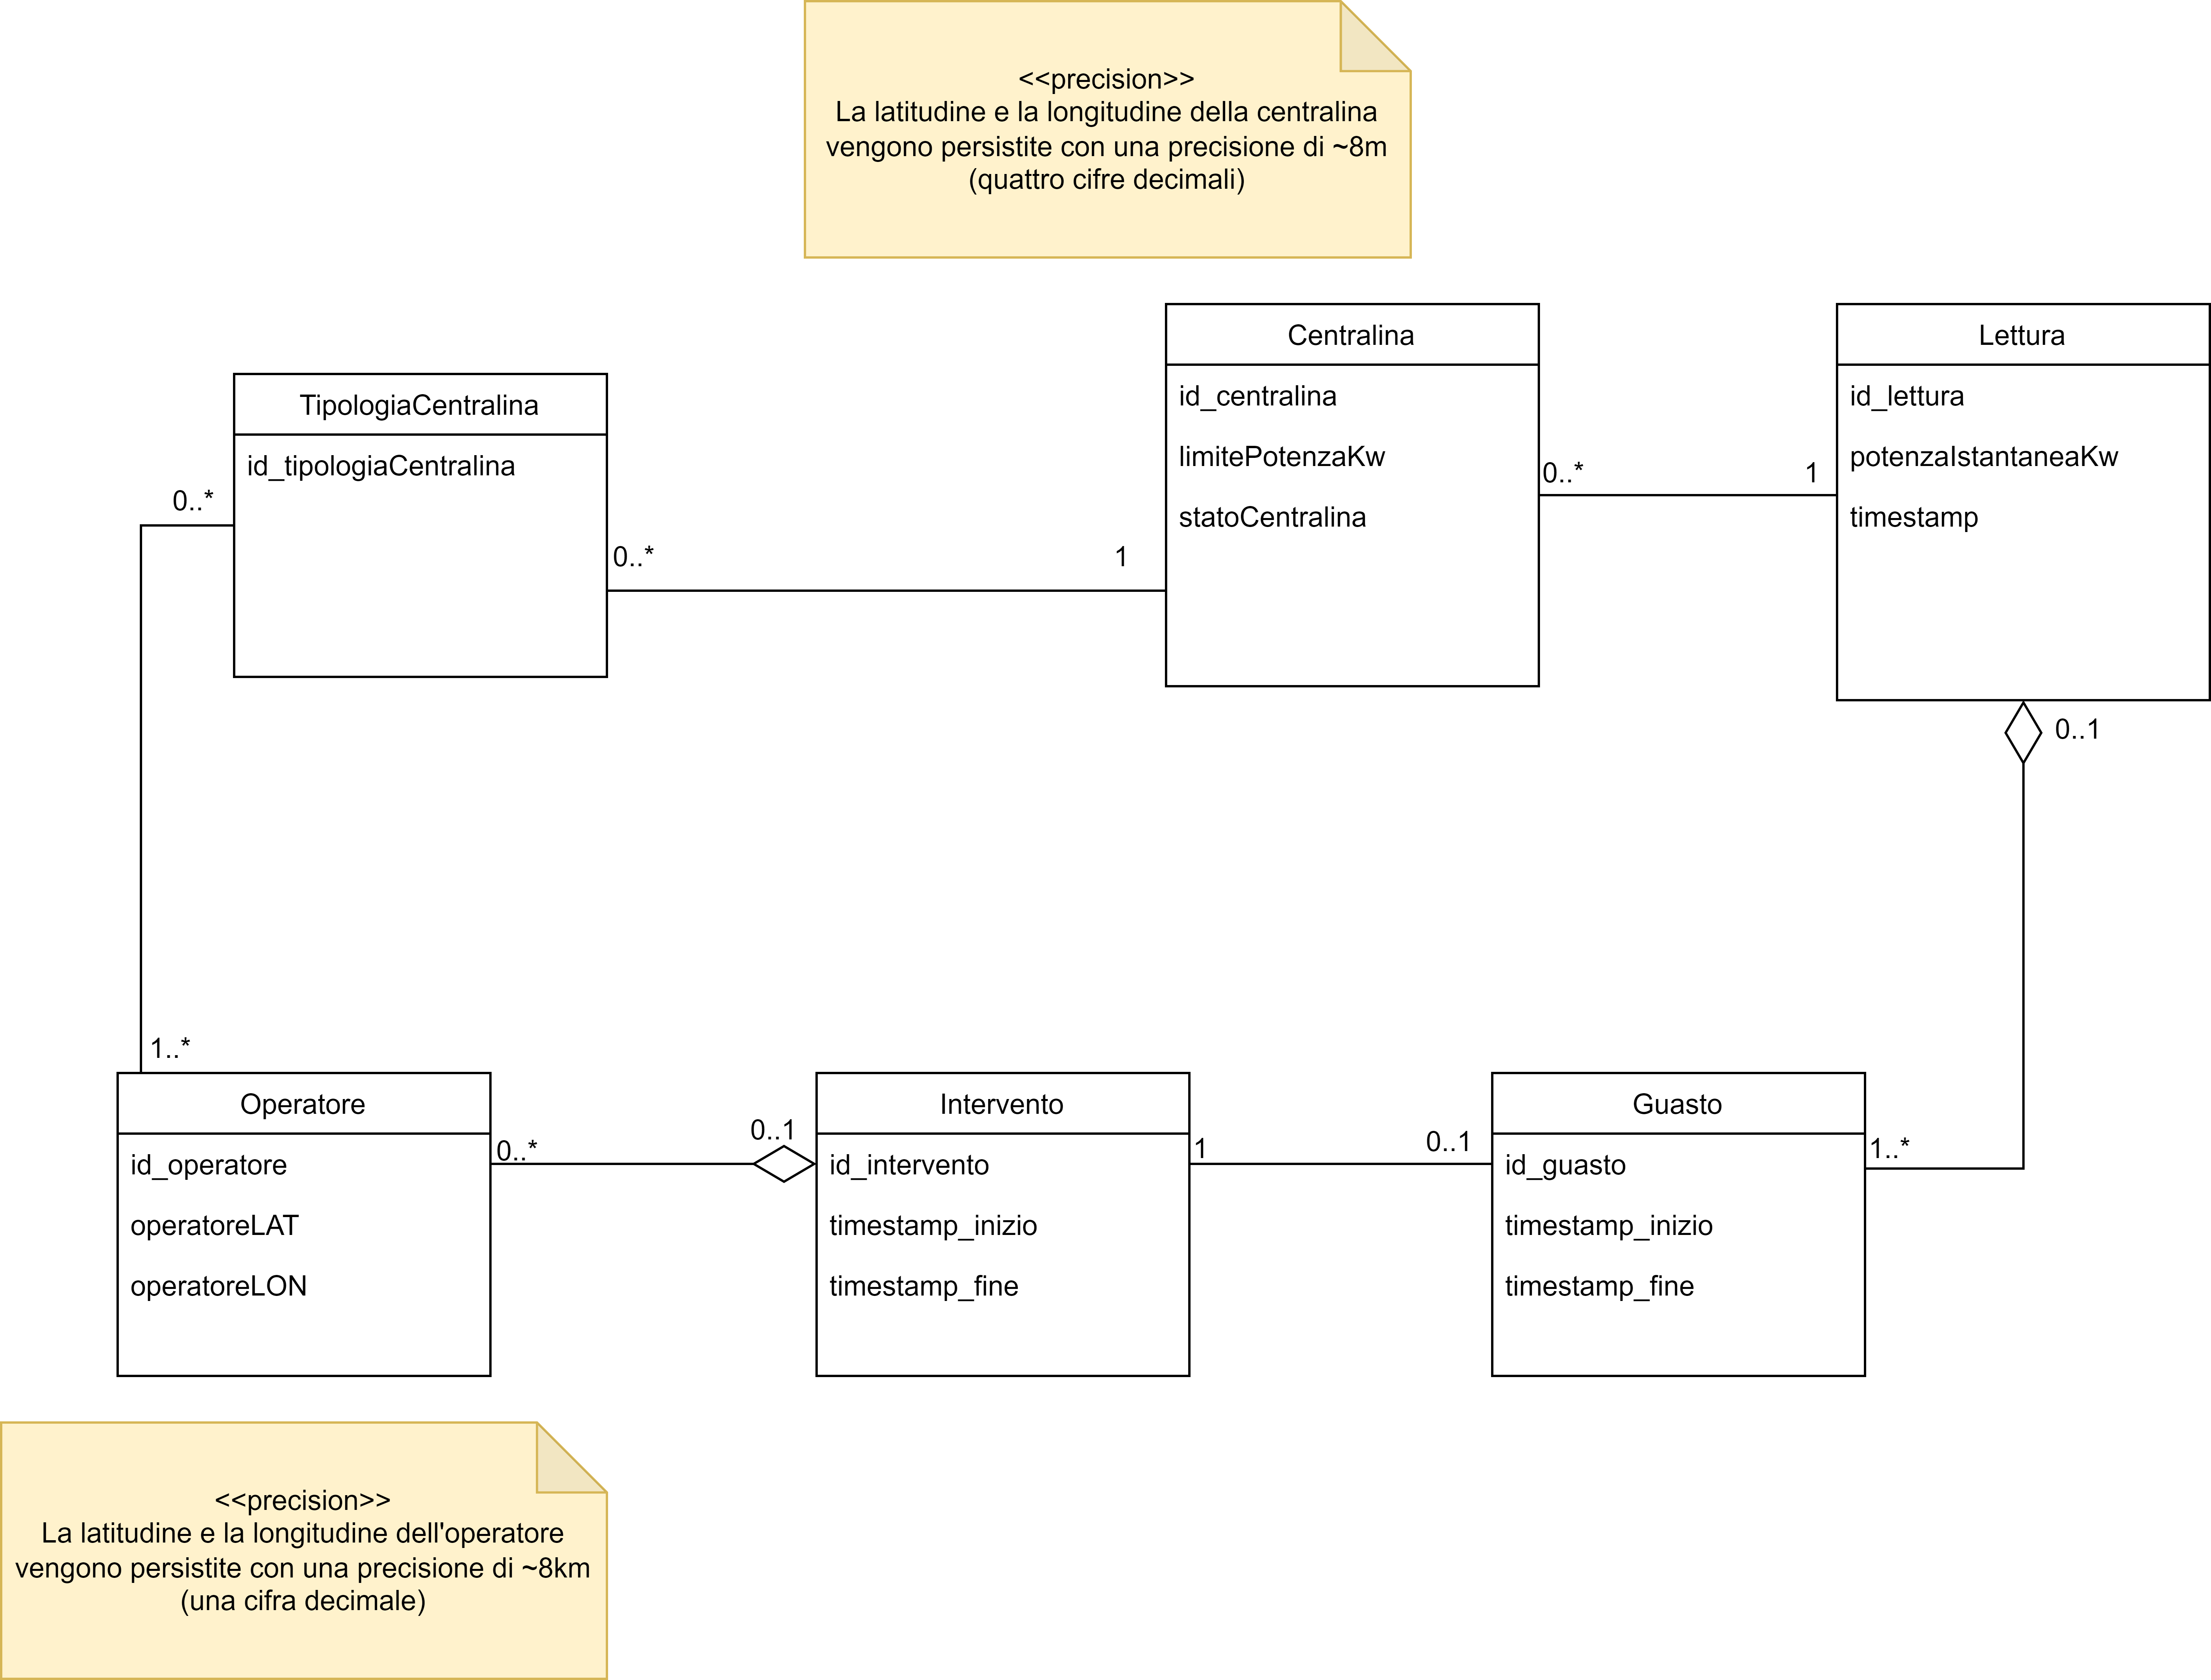
\includegraphics[width=0.85\textwidth, height=\textheight, keepaspectratio=true]{domain_model.png}
		\end{center}
	\end{frame}
	
	\subsection{Diagramma dei casi d'uso}\label{use_cases_diagram}
	\begin{frame}
		\frametitle{\nameref{use_cases_diagram}}
		\begin{center}
			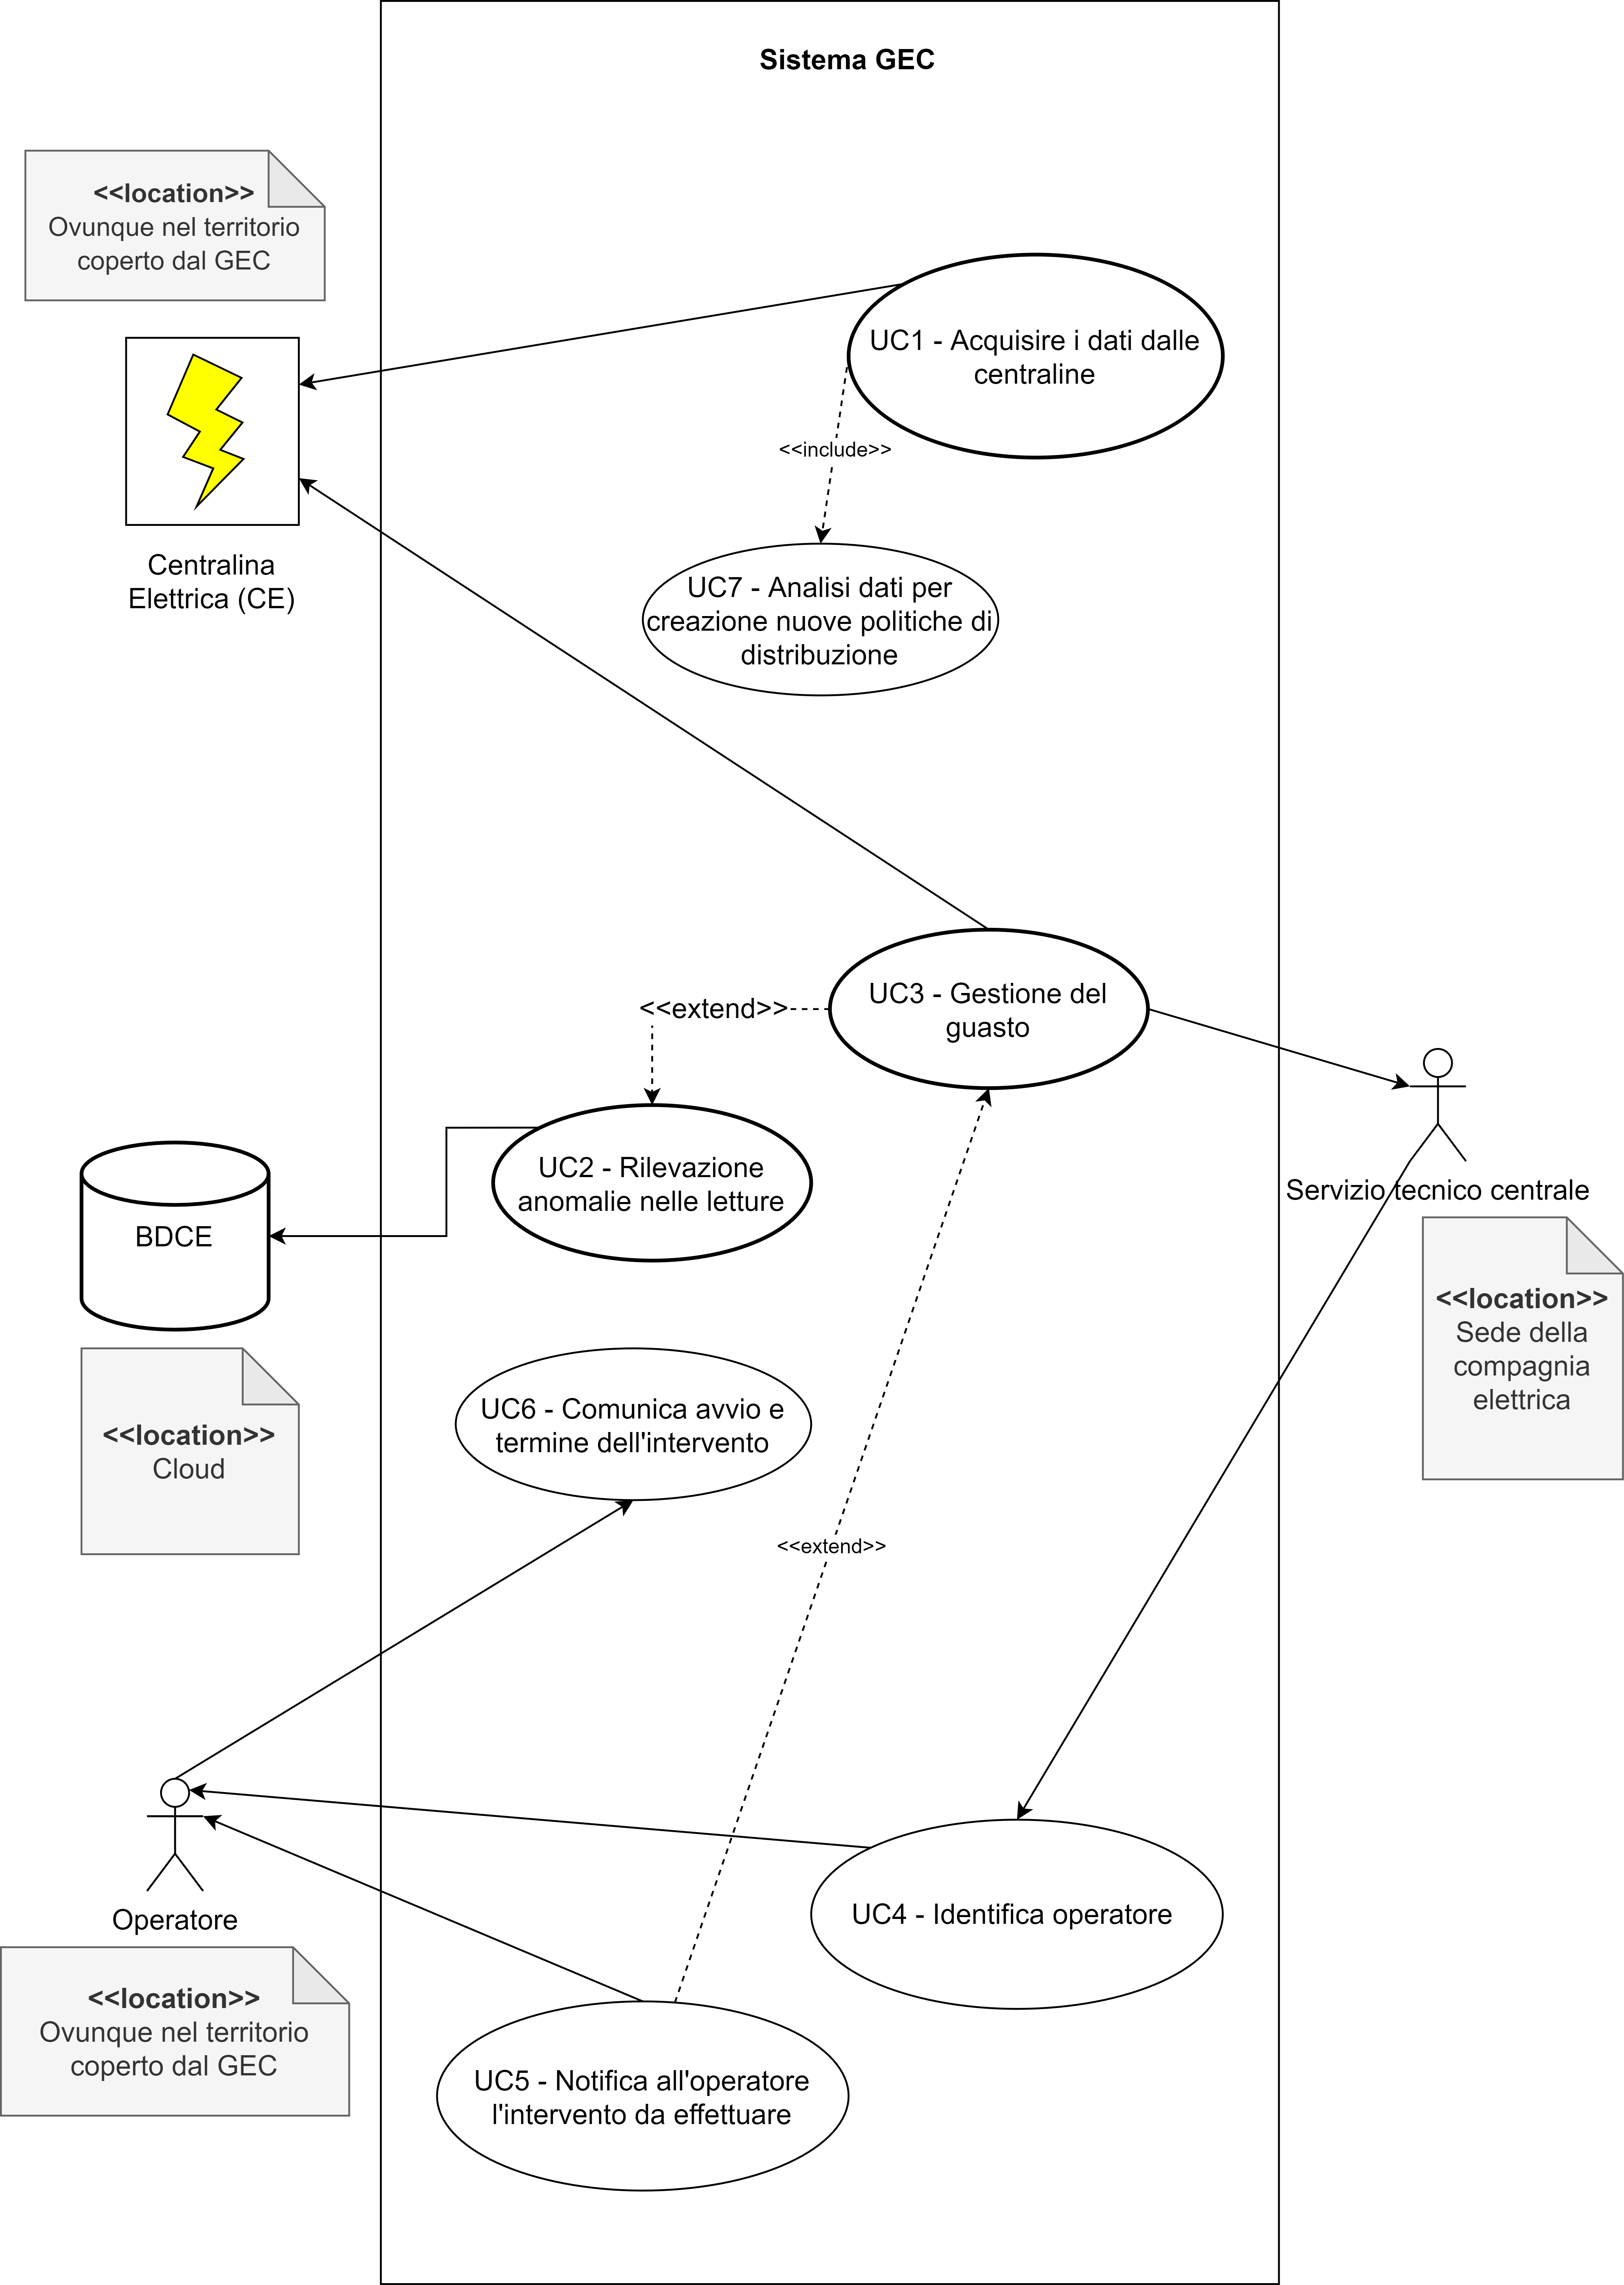
\includegraphics[width=\textwidth, height=0.85\textheight, keepaspectratio=true]{use_cases_diagram.png}
		\end{center}
	\end{frame}

	\subsection{Diagrammi delle attività}\label{activity_diagram}
		\begin{frame}	
		\frametitle{\nameref{use_cases_diagram}}
		\begin{block}{\nameref{use_cases_diagram}}
			\begin{itemize}
				\item ADUC1 - Acquisire dati centraline
				\item ADUC2 - Rilevazione anomalie nelle letture
				\item ADUC3 - Gestione del guasto
				\item ADUC4 - Identifica operatore
				\item ADUC5 - Notifica all'operatore l'intervento da effettuare
				\item ADUC6 - Comunica avvio e termine dell'intervento
				\item ADUC7 - Analisi dati per creazione nuove politiche di distribuzione
			\end{itemize}
		\end{block}
		\end{frame}
		
		\begin{frame}
	    \subsubsection{ADUC1 - Acquisire dati centraline}	 
		\begin{block}{ADUC1 - Acquisire dati centraline}
			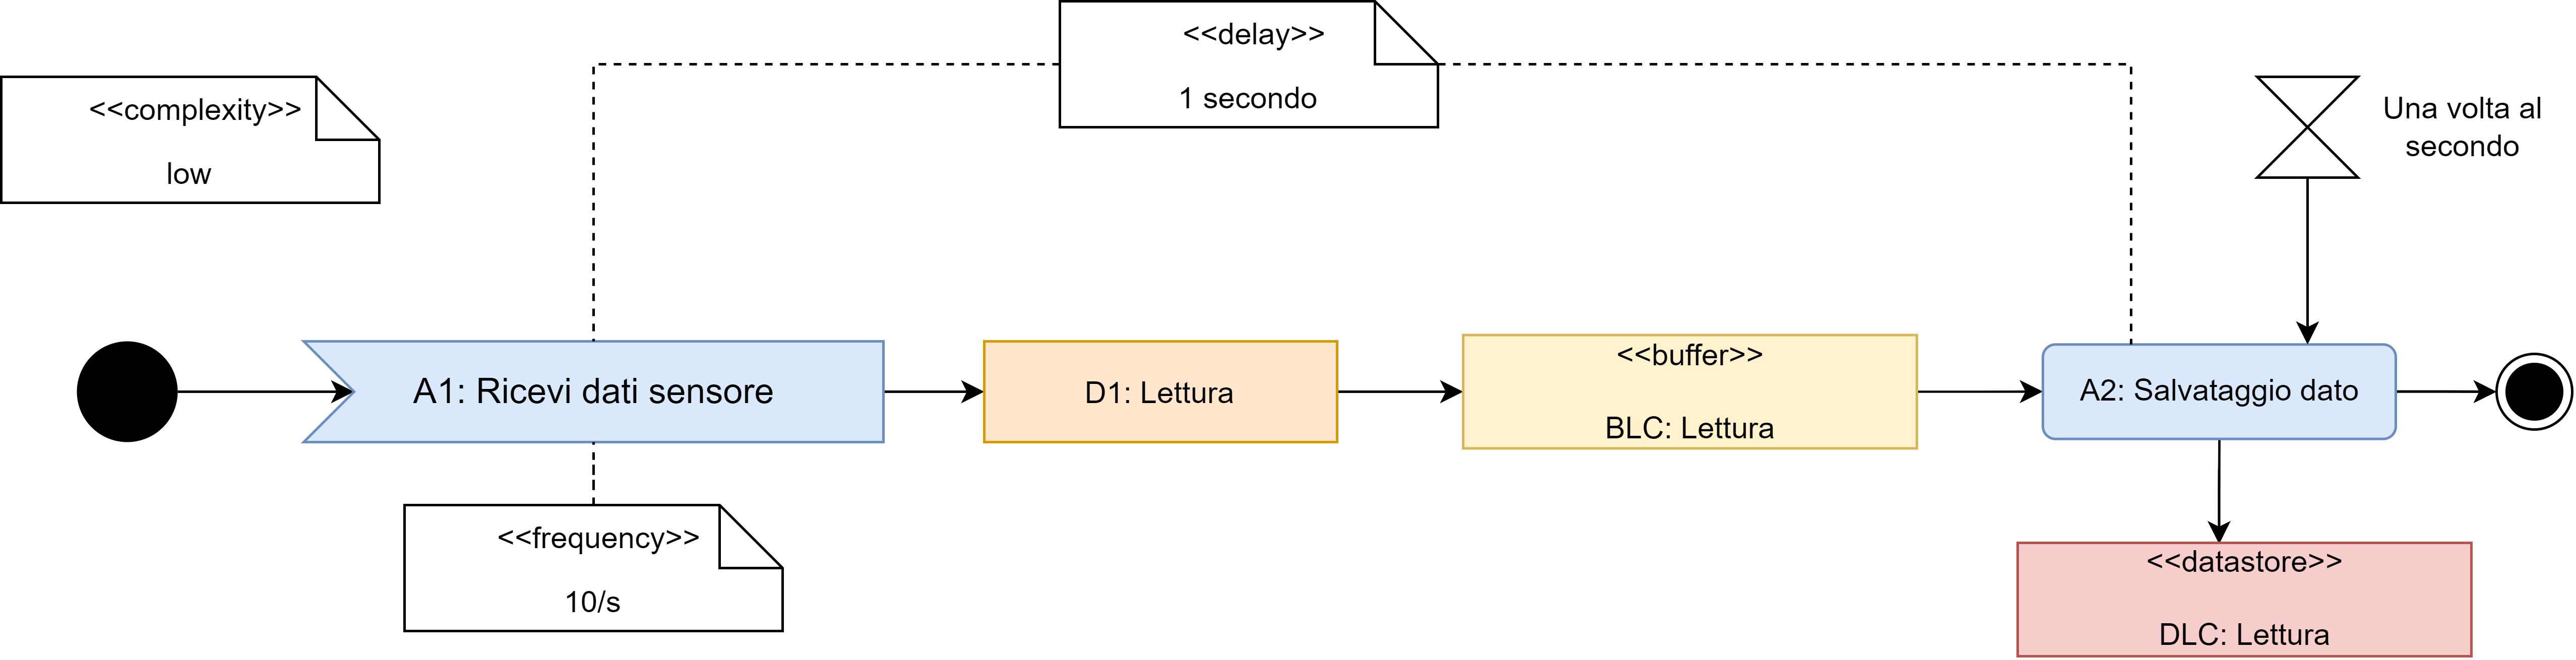
\includegraphics[width=\textwidth, height=0.85\textheight, keepaspectratio=true]{ADUC1.png}
		\end{block}
		\end{frame}

		
		\begin{frame}
		\subsubsection{ADUC2 - Rilevazione anomalie nelle letture}		
		\begin{block}{ADUC2 - Rilevazione anomalie nelle letture}
			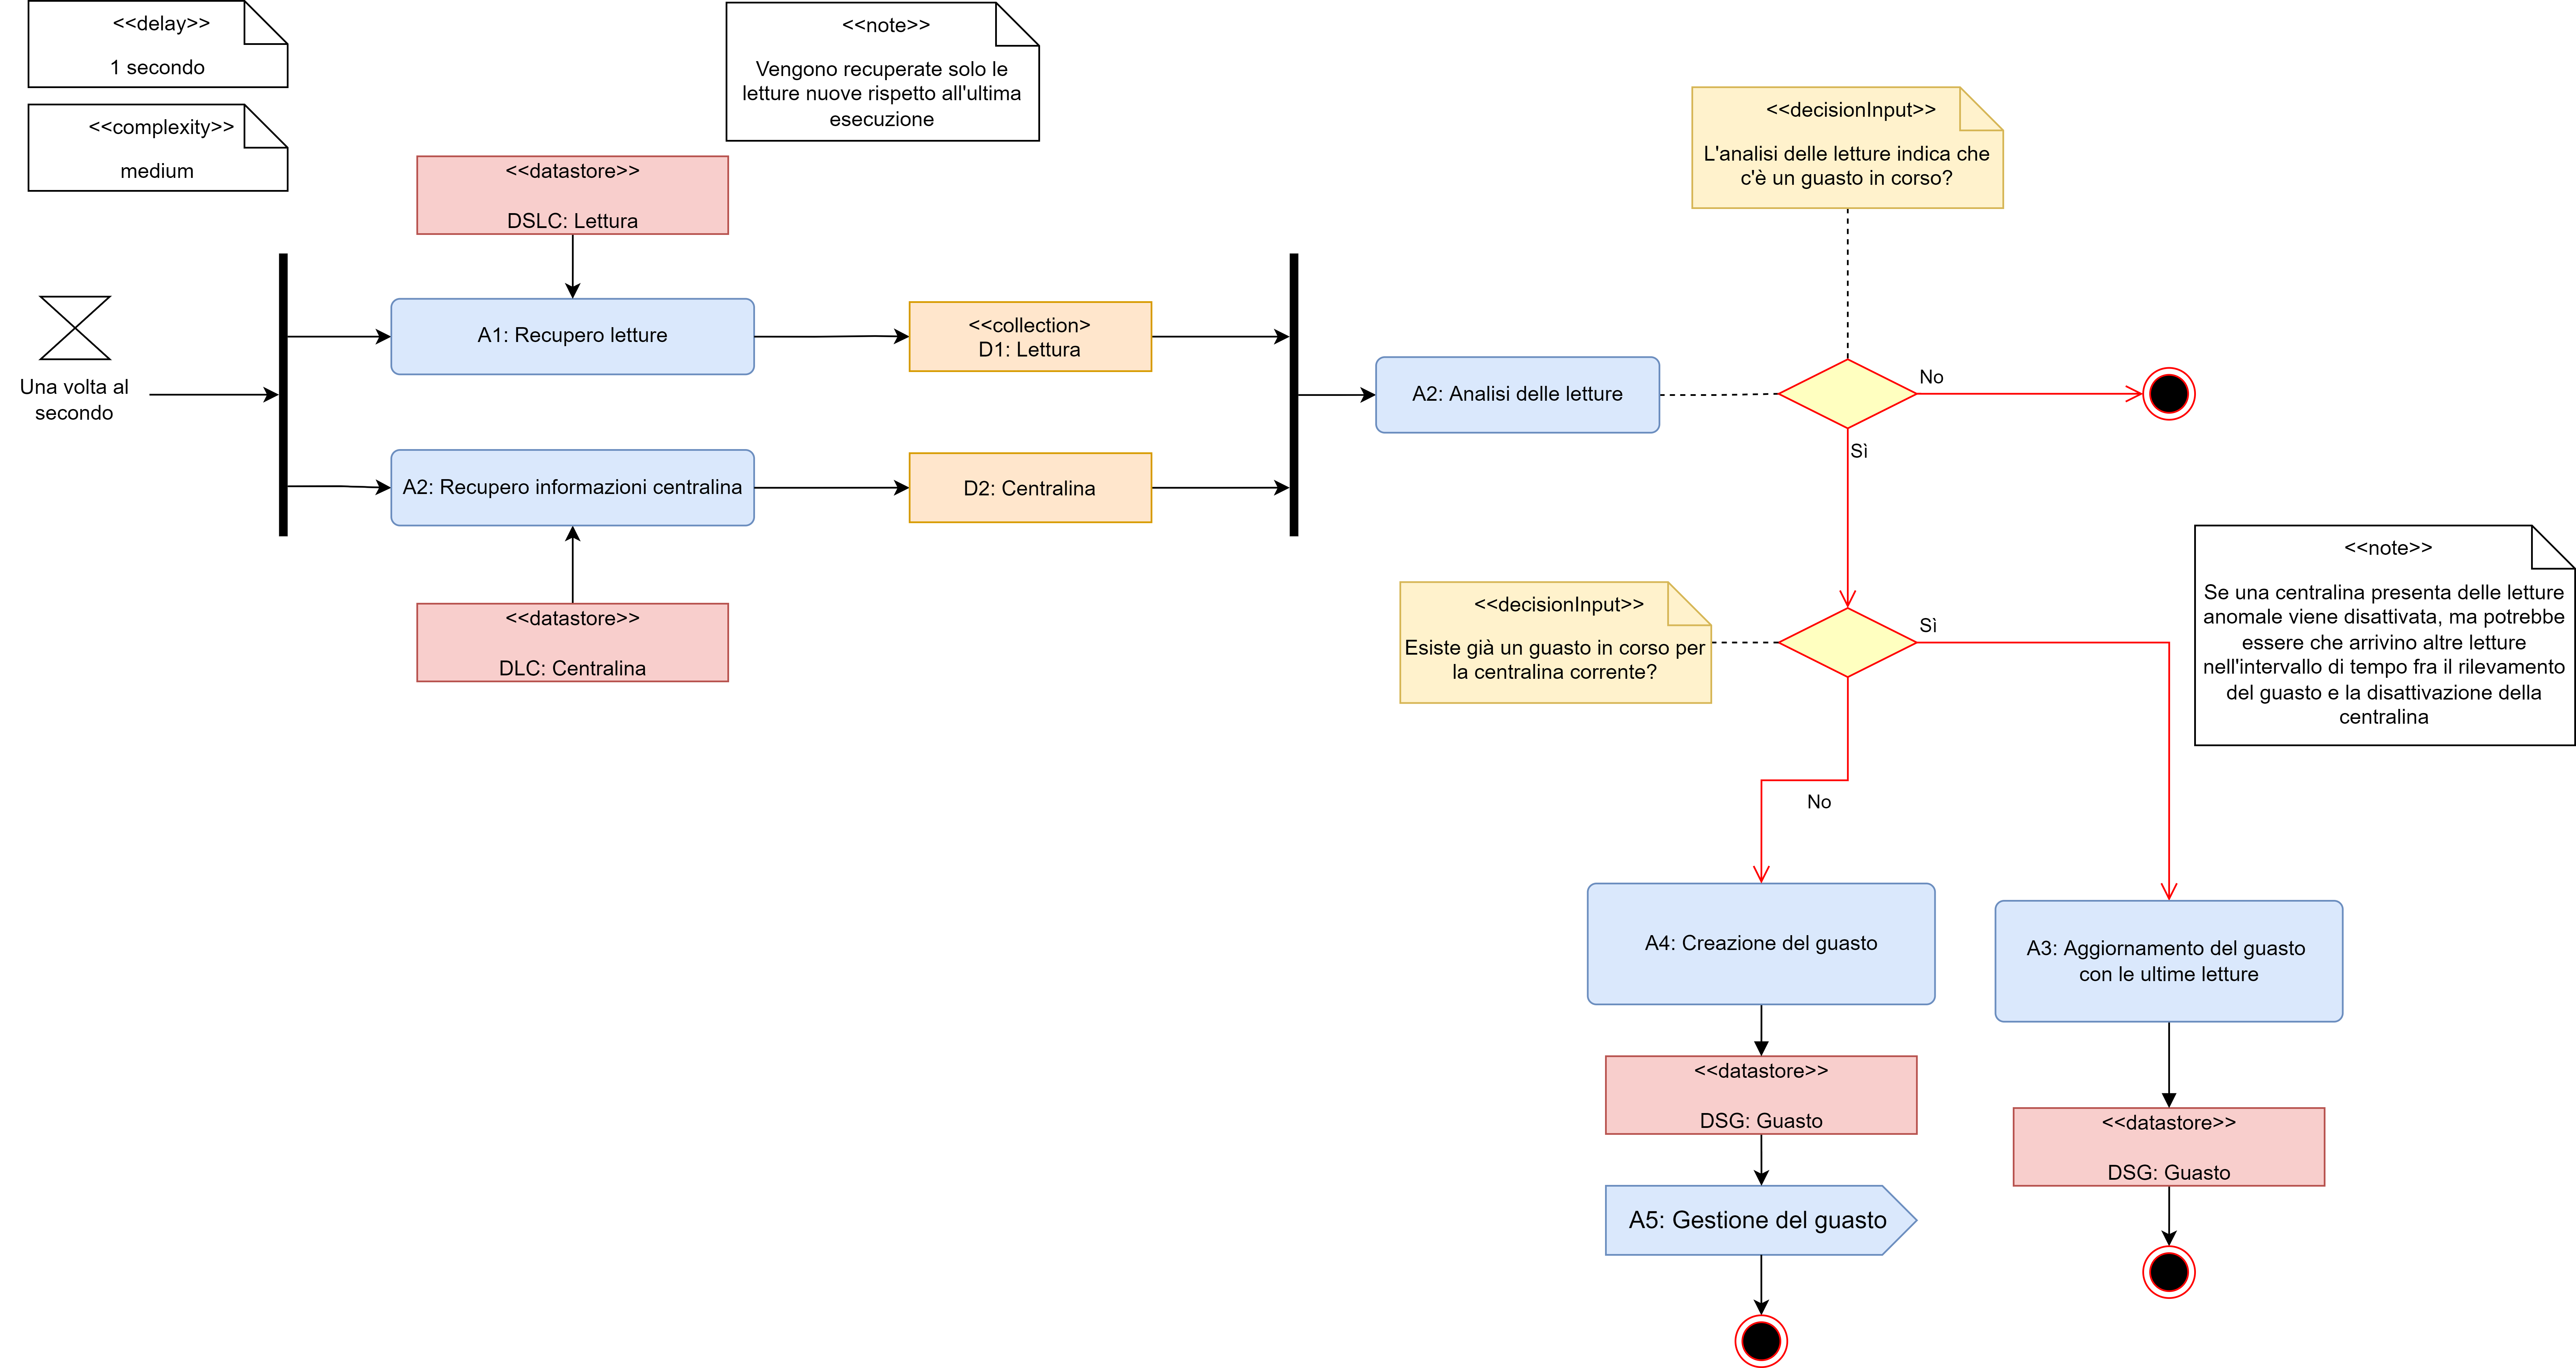
\includegraphics[width=\textwidth, height=0.85\textheight, keepaspectratio=true]{ADUC2.png}
		\end{block}
		\end{frame}

	
		\begin{frame}
		\subsubsection{ADUC3 - Gestione del guasto}	
			\begin{block}{ADUC3 - Gestione del guasto}
				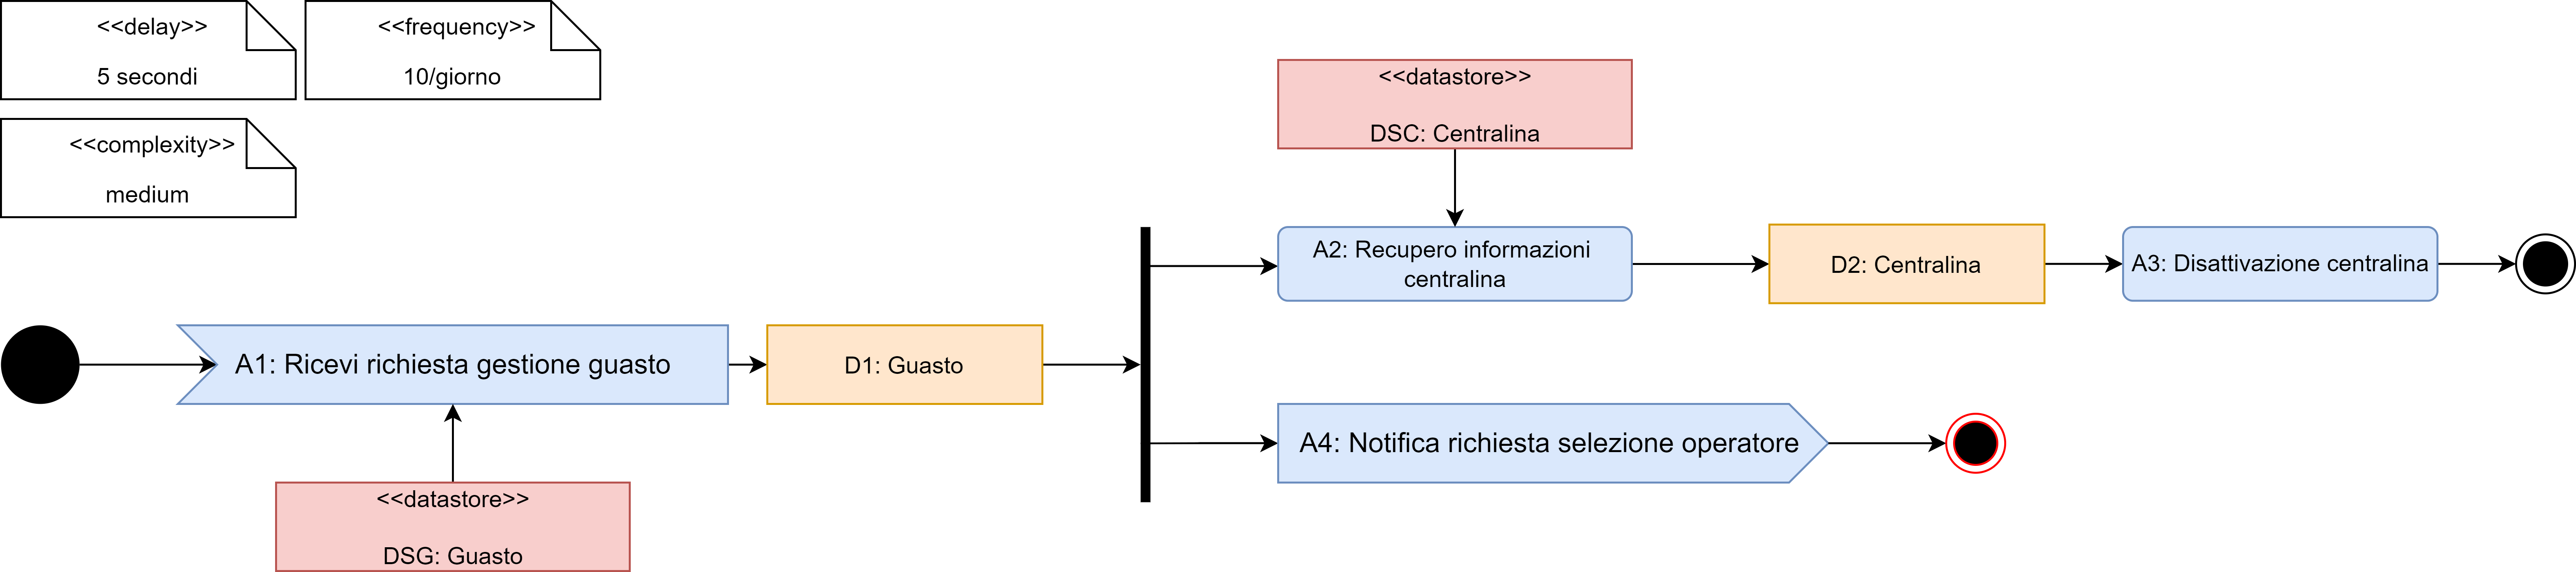
\includegraphics[width=\textwidth, height=0.85\textheight, keepaspectratio=true]{ADUC3.png}
			\end{block}
		\end{frame}
	
		\begin{frame}
		\subsubsection{ADUC4 - Identifica operatore}	
			\begin{block}{ADUC4 - Identifica operatore}
				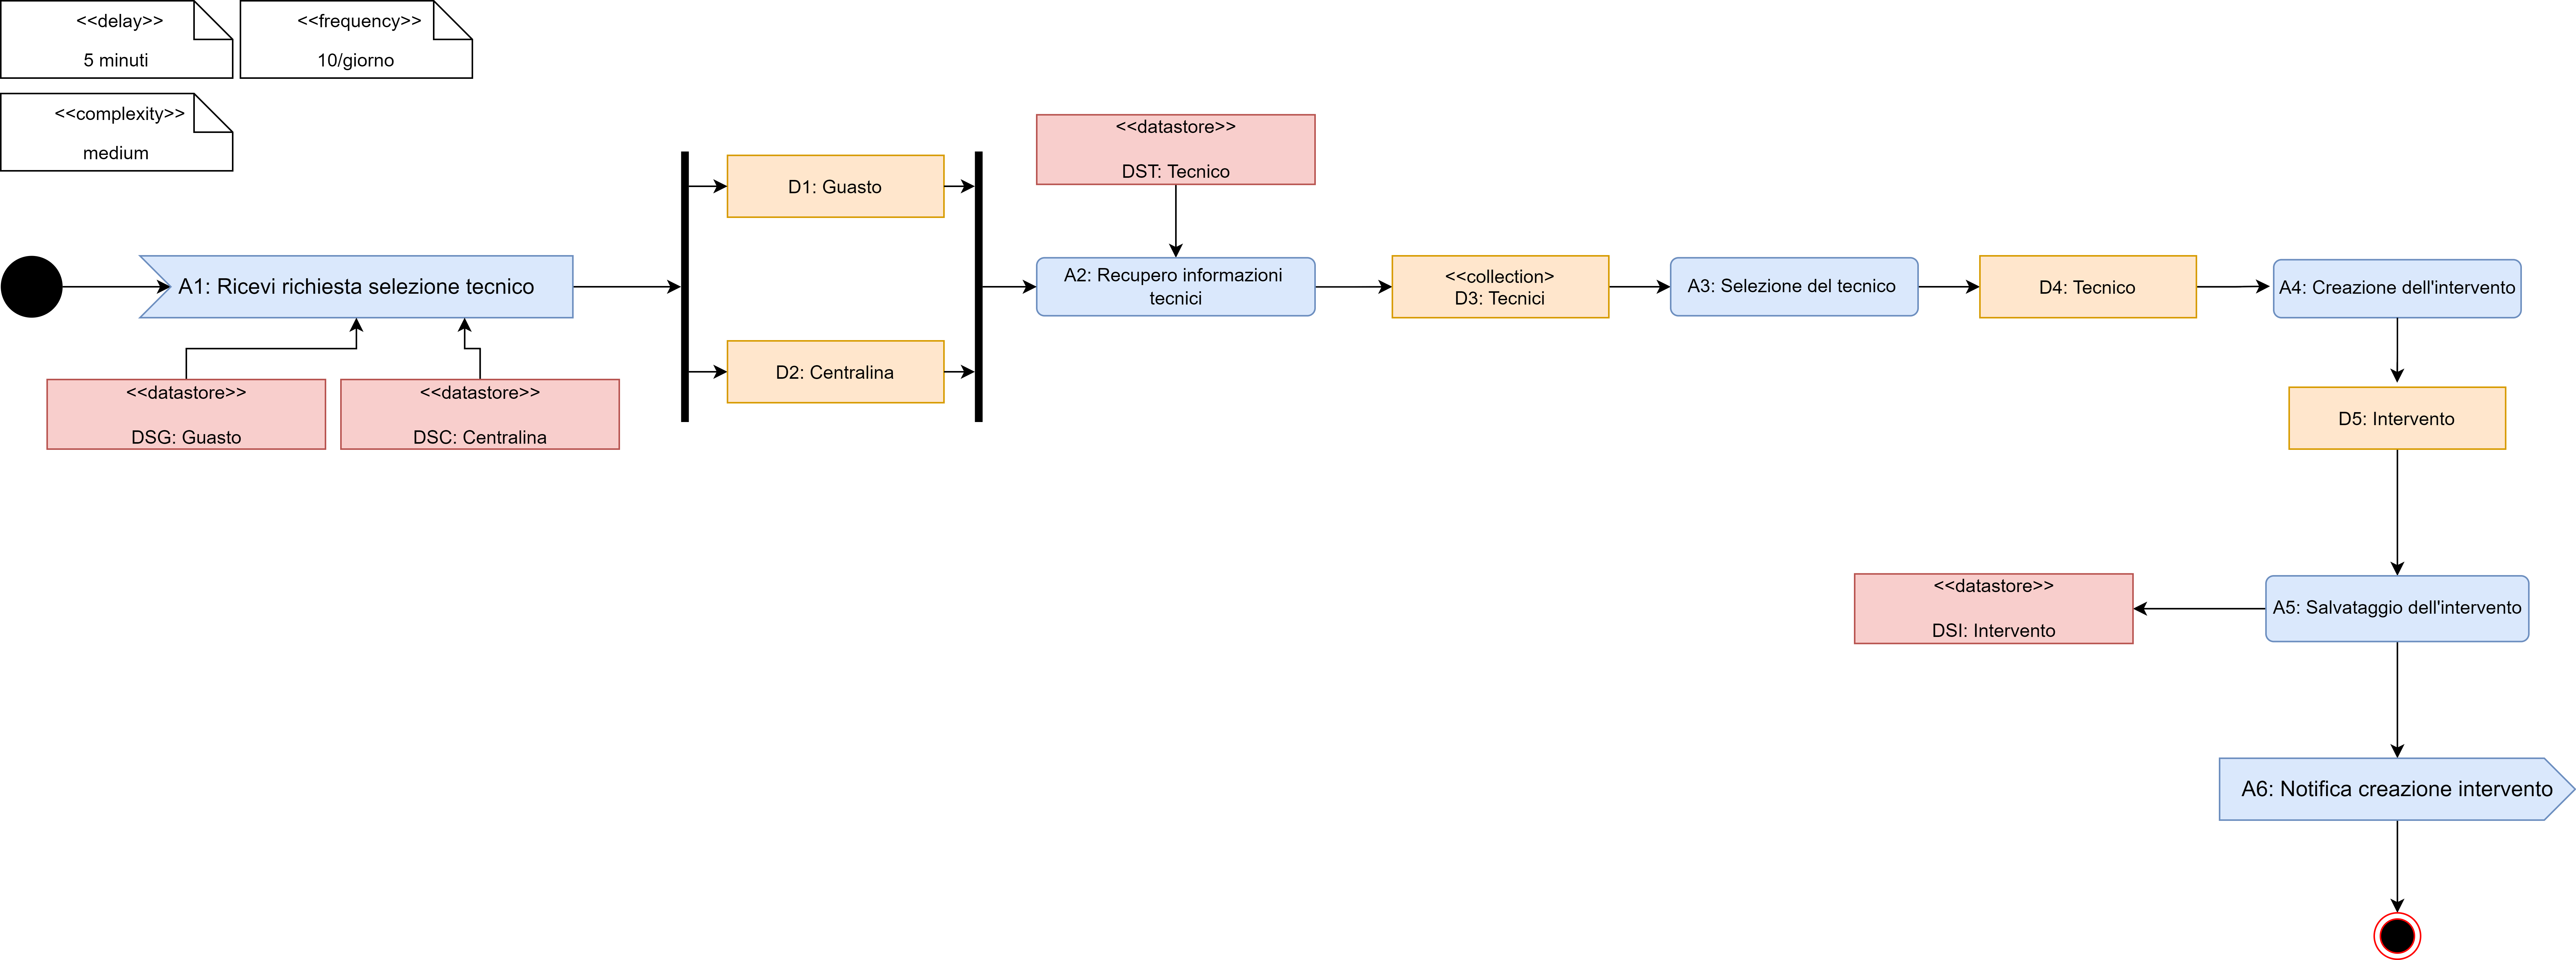
\includegraphics[width=\textwidth, height=0.85\textheight, keepaspectratio=true]{ADUC4.png}
			\end{block}
		\end{frame}

		\begin{frame}
		\subsubsection{ADUC5 - Notifica all'operatore}	
			\begin{block}{ADUC5 - Notifica all'operatore l'intervento da effettuare}
				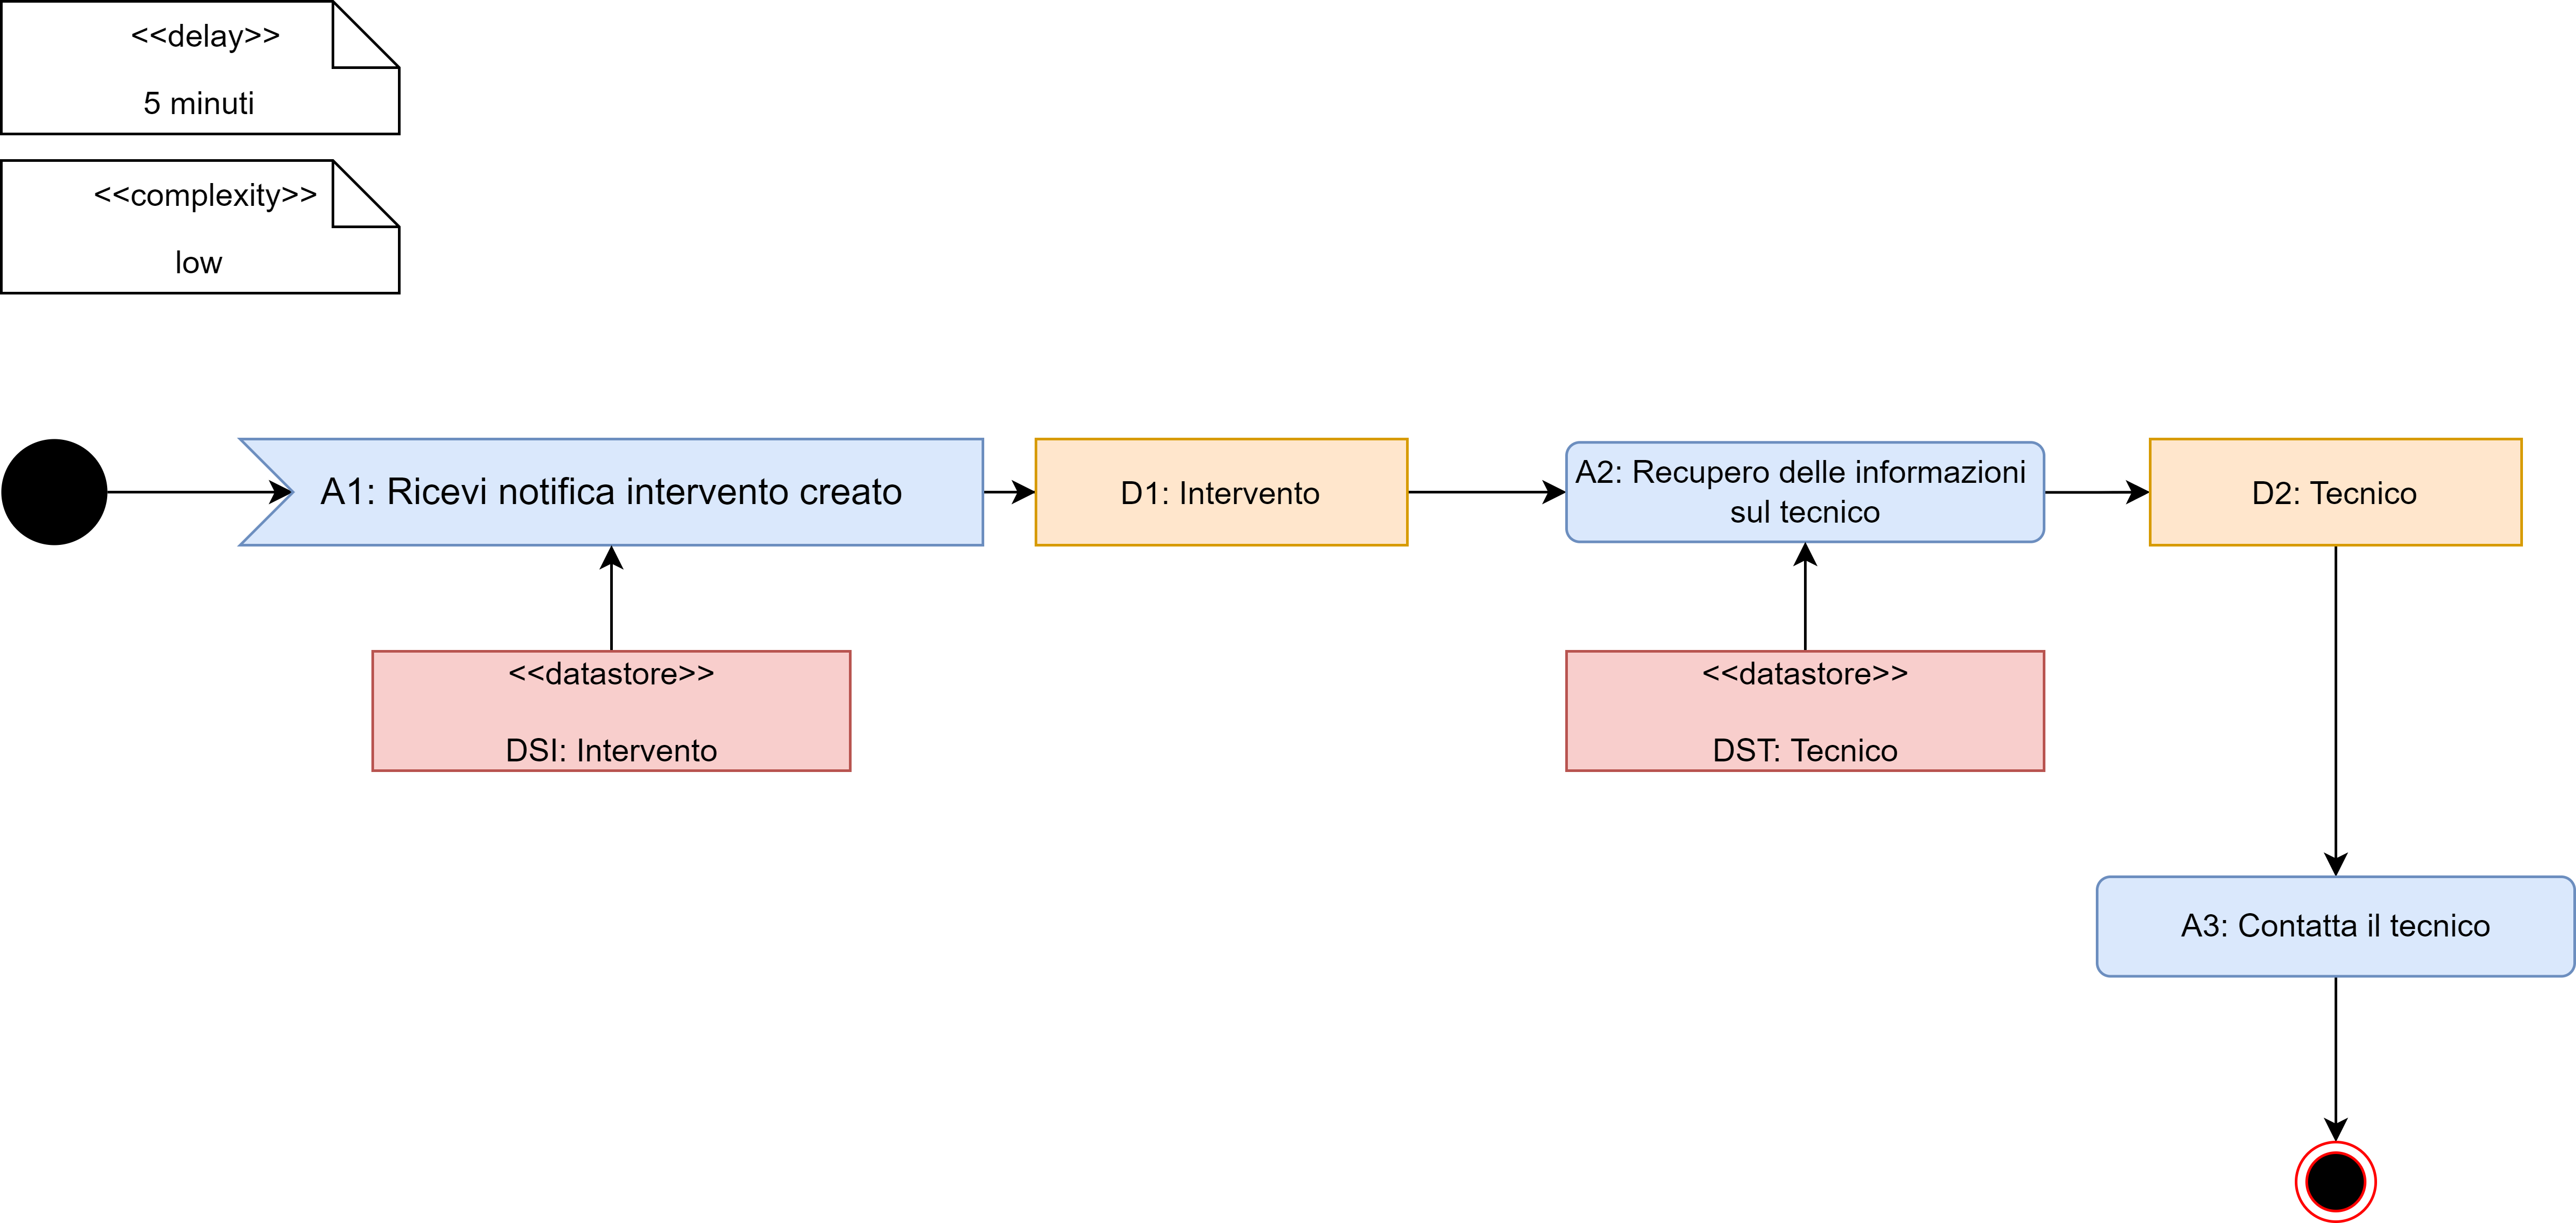
\includegraphics[width=\textwidth, height=0.85\textheight, keepaspectratio=true]{ADUC5.png}
			\end{block}
		\end{frame}	

		\begin{frame}
		\subsubsection{ADUC6 - Comunica avvio e termine dell'intervento}			
			\begin{block}{ADUC6 - Comunica avvio e termine dell'intervento}
				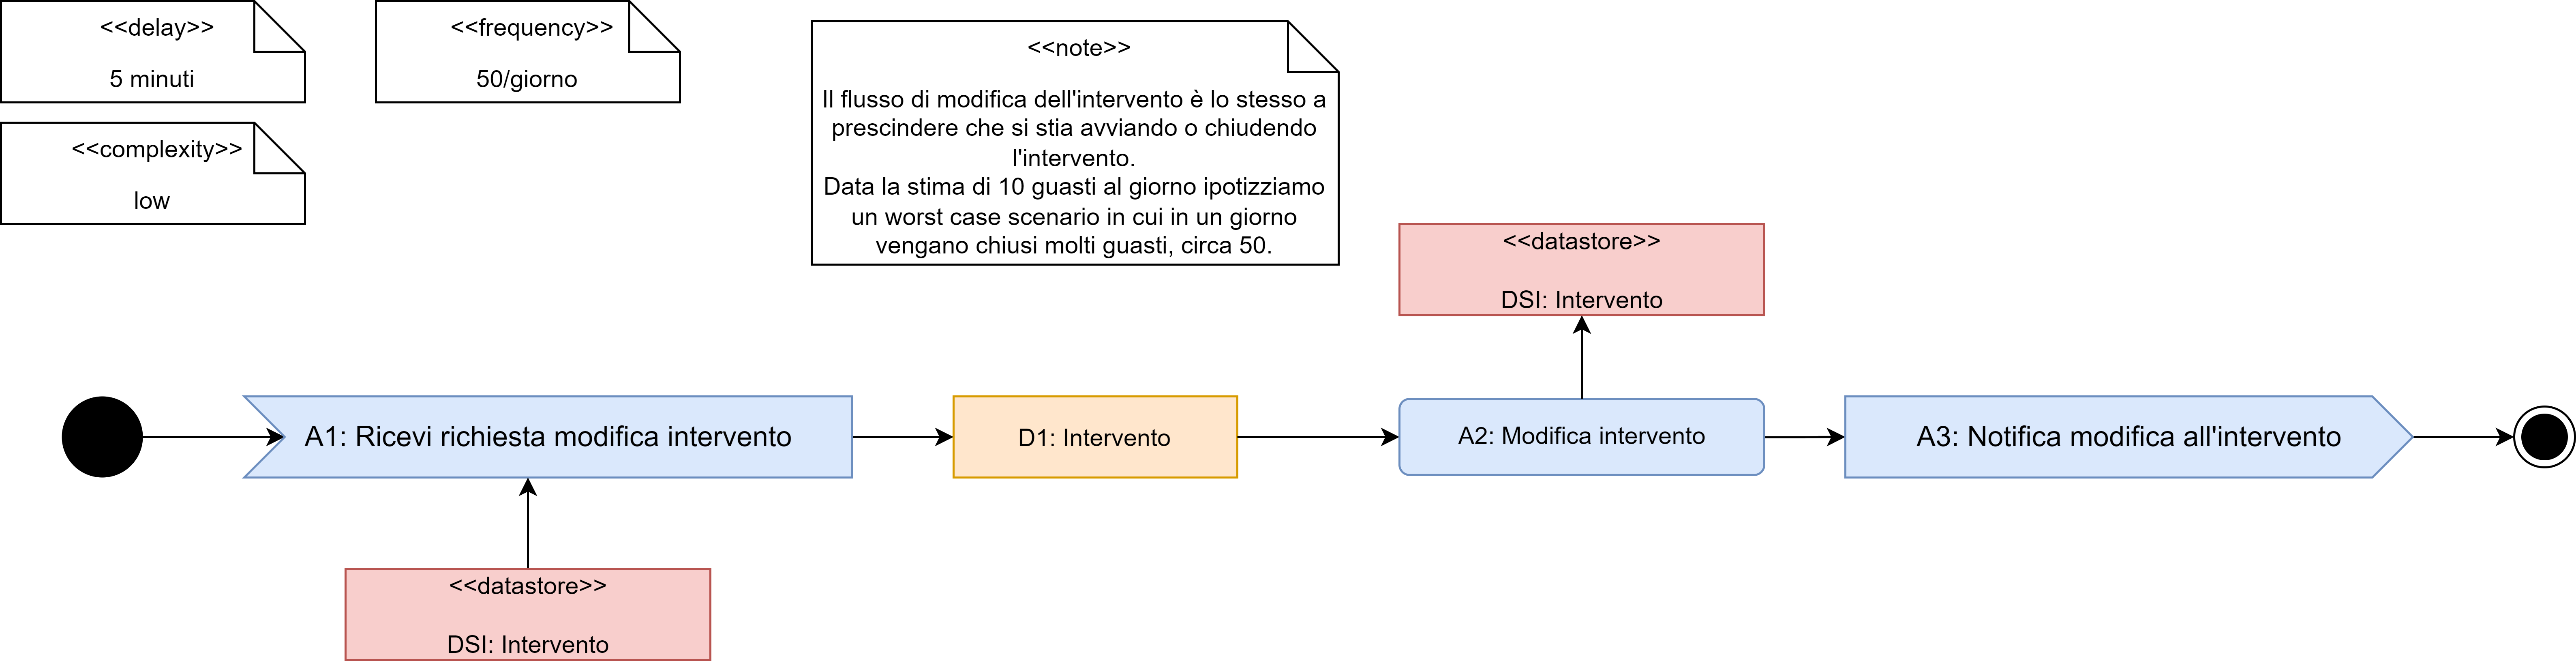
\includegraphics[width=\textwidth, height=0.85\textheight, keepaspectratio=true]{ADUC6.png}
			\end{block}
		\end{frame}	
	
		\begin{frame}
		\subsubsection{ADUC7 - Analisi dati per creazione nuove politiche di distribuzione}			
			\begin{block}{ADUC7 - Analisi dati per creazione nuove politiche di distribuzione}
				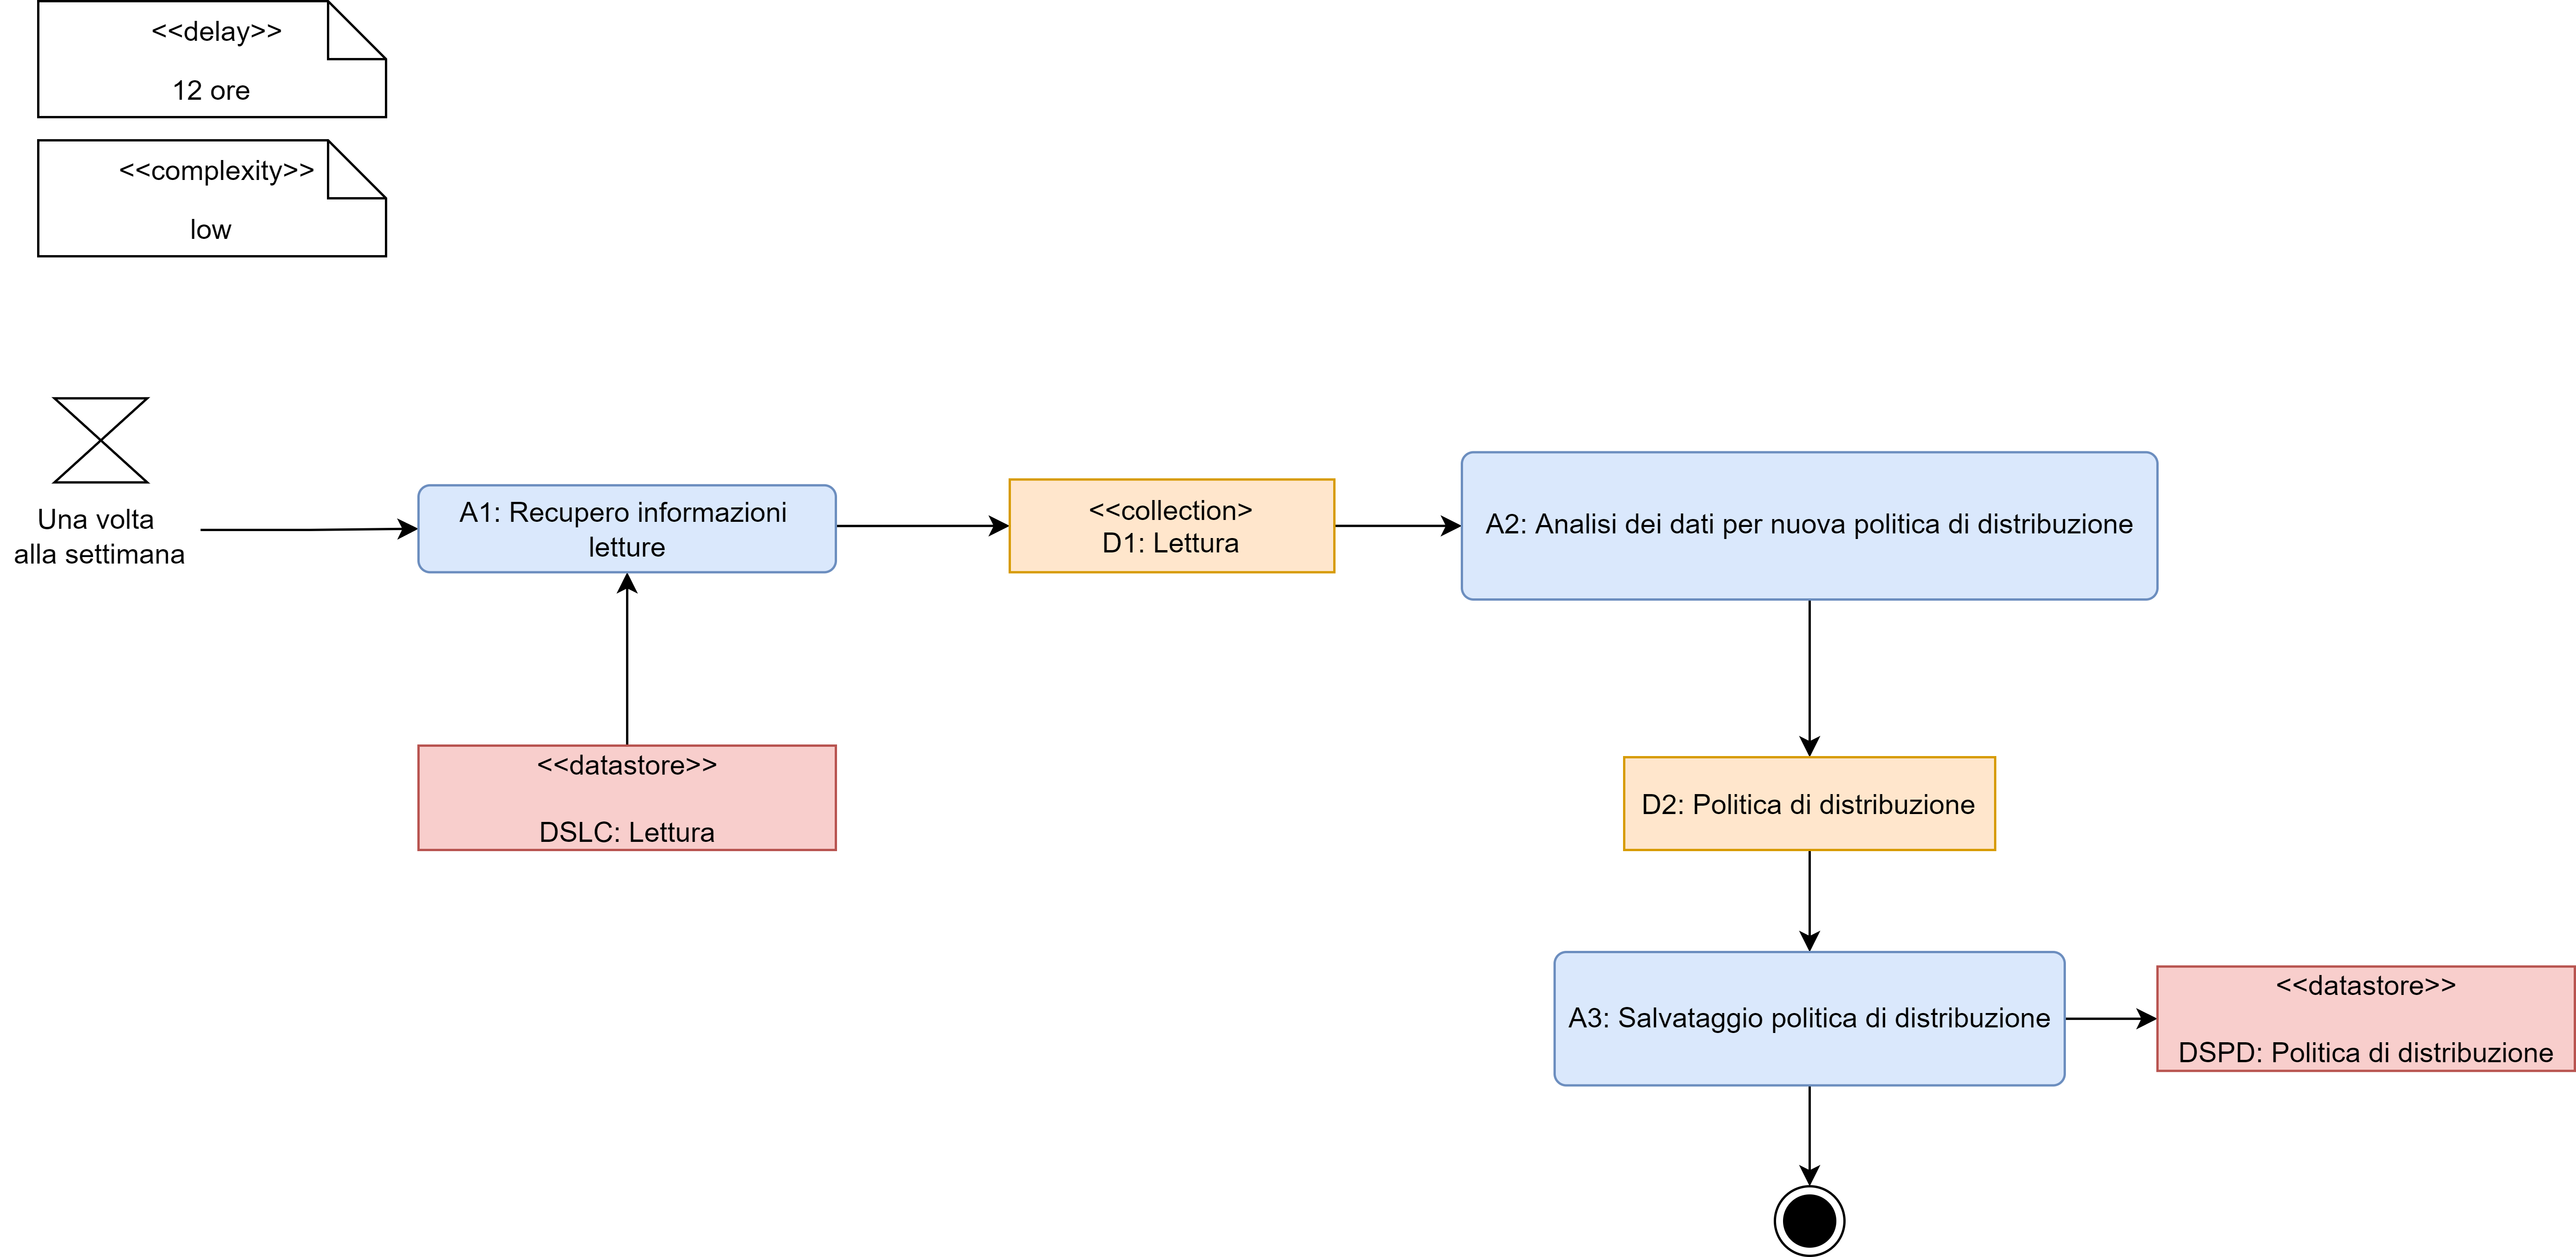
\includegraphics[width=\textwidth, height=0.85\textheight, keepaspectratio=true]{ADUC7.png}
			\end{block}
		\end{frame}	
	
	\section{Architettura logica}
	\subsection{Valori dimensionali architetturali strutturali}\label{val_dim_arch_strut}
	
	\begin{frame}
		\frametitle{\nameref{val_dim_arch_strut}}			
		\begin{center}
				\begin{table}
				\centering
				{\renewcommand{\arraystretch}{1.5}
				\begin{tabular}{|c|M{0.4\textwidth}|c|}
					\hline
					\rowcolor{intestazione}
					Dimensione & Valori ammissibili & \#Valori ammissibili \\
					\hline
					\rowcolor{riga1}
					Complessità & low, medium & 2 \\
					\rowcolor{riga2}
					Frequency & 10/s, 1/s, 10/giorno, 50/giorno, 1/settimana & 5 \\
					\rowcolor{riga1}
					Delay & 1s, 5s, 5 minuti, 12 ore & 4 \\
					\rowcolor{riga2}
					Abstraction & Centralina, Lettura,  Guasto,  Intervento, Operatore,  Politica di distribuzione   & 6 \\
					\rowcolor{riga1}
					Location & Cloud, Ovunque nel territorio coperto dal GEC, Sede della compagnia elettrica & 3 \\
					\hline
				\end{tabular}}
			\end{table}
		\end{center}
	
	\end{frame}	

	\subsection{Partizionamento
		per funzionalità}\label{part_funz}
	\begin{frame}
		\frametitle{\nameref{part_funz}}
		\begin{block}{\nameref{part_funz}}
		 	\begin{enumerate}
		 		\item Gestore acquisizione dati centralina
		 		\begin{itemize}
		 			\item ADUC1
		 		\end{itemize}
	 			\item Gestore guasti
	 			\begin{itemize}
	 				\item ADUC2
	 				\item ADUC3
	 			\end{itemize}
 				\item Gestore interventi
 				\begin{itemize}
 					\item ADUC4
 					\item ADUC5
 					\item ADUC6
 				\end{itemize}
 			 	\item Gestore politiche di distribuzione
 				\begin{itemize}
					\item ADUC7
 				\end{itemize}
		 	\end{enumerate}
		\end{block}
	\end{frame}


	\begin{frame}
	\subsubsection{Gestore acquisizione dati centralina}	
	\begin{block}{Gestore acquisizione dati centralina}
		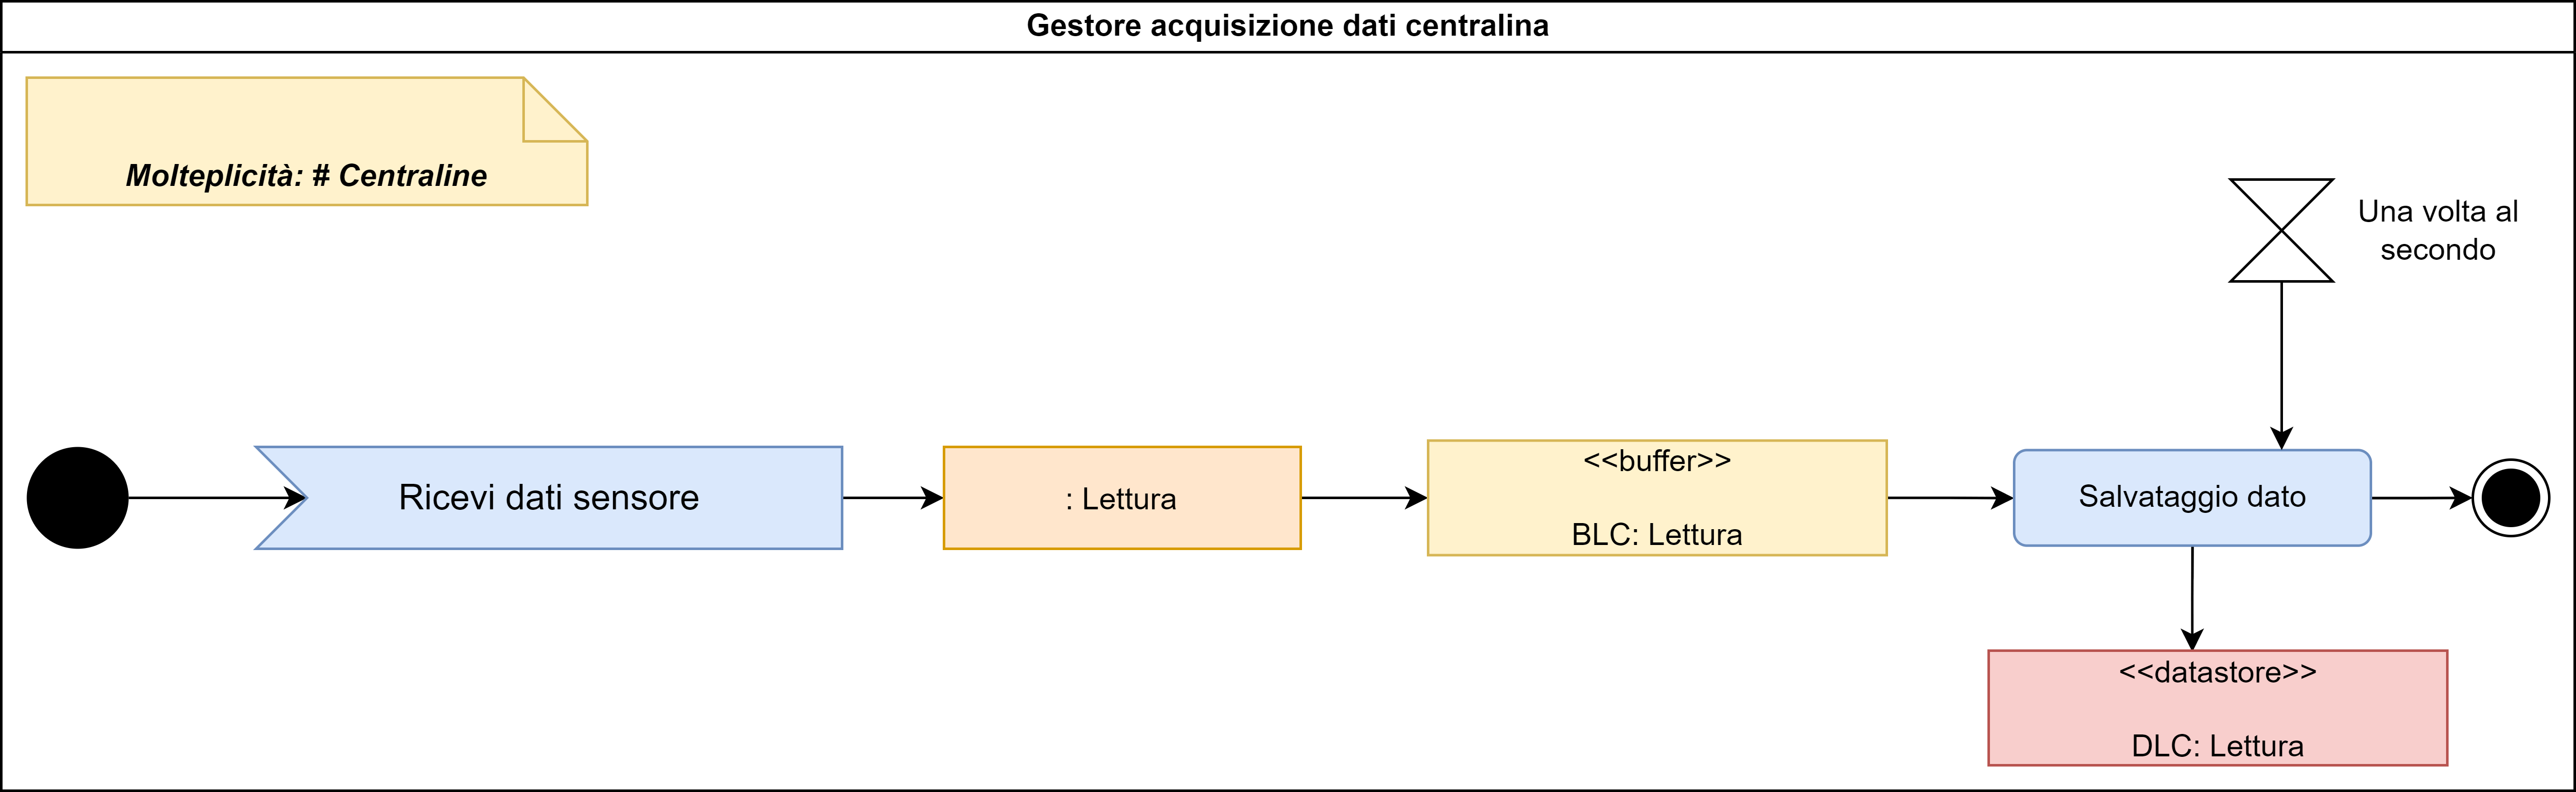
\includegraphics[width=\textwidth, height=0.85\textheight, keepaspectratio=true]{comp1.png}
	\end{block}
	\end{frame}	

	\begin{frame}
		\subsubsection{Gestore guasti}	
		\begin{block}{Gestore guasti}
			\includegraphics[width=\textwidth, height=0.85\textheight, keepaspectratio=true]{comp2.png}
		\end{block}
	\end{frame}	
	
	\begin{frame}
		\subsubsection{Gestore interventi}	
		\begin{block}{Gestore interventi}
			\includegraphics[width=\textwidth, height=0.85\textheight, keepaspectratio=true]{comp3.png}
		\end{block}
	\end{frame}	
	
	\begin{frame}
		\subsubsection{Gestore politiche di distribuzione}	
		\begin{block}{Gestore politiche di distribuzione}
			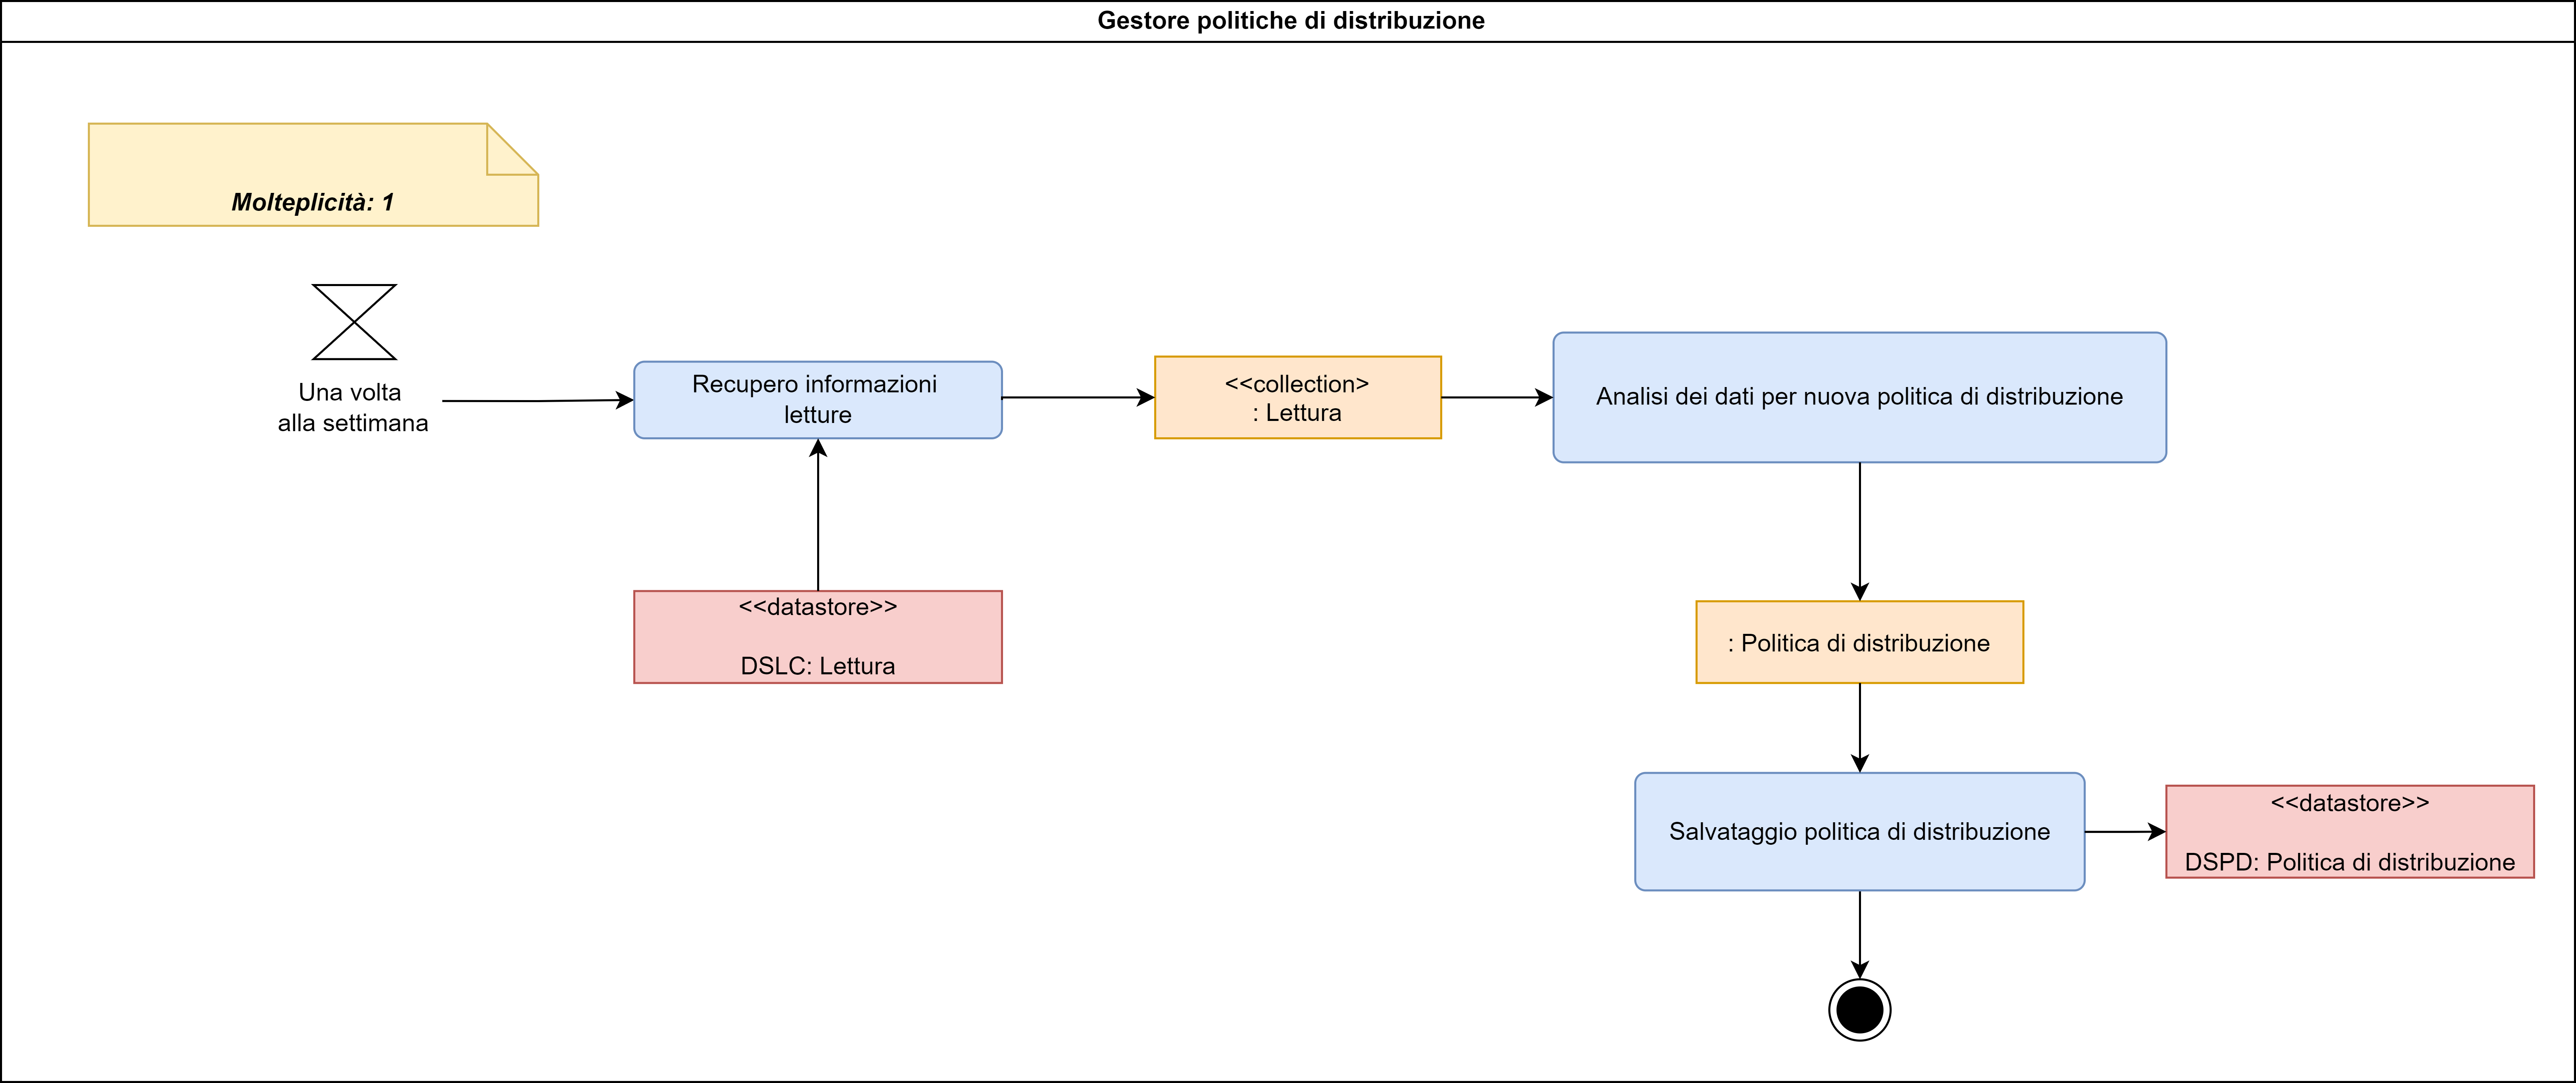
\includegraphics[width=\textwidth, height=0.85\textheight, keepaspectratio=true]{comp4.png}
		\end{block}
	\end{frame}	
	
	\subsubsection{Dimensioni statiche}
		\begin{frame}[allowframebreaks]
		\frametitle{Dimensioni statiche}			
		\begin{center}
			\begin{table}
				\tiny
				\centering
				{\renewcommand{\arraystretch}{1.2}
					
					\begin{tabular}{|M{0.1\textwidth}|M{0.1\textwidth}|p{.6\textwidth}|}
						\hline
						\rowcolor{intestazione}
						Dimensione & Valore & Commenti \\
						\hline
						\rowcolor{riga1}
						Complexity & 25 & Le complessità delle attività nelle componenti sono omogenee:
						\begin{itemize}
								\item Gestore acquisizione dati centralina : low
								\item Gestore guasti: 1 low, 1 medium
								\item Gestore interventi: 2 low, 1 medium
								\item Gestore politiche di distribuzione: 1 low
						\end{itemize} \\
						\rowcolor{riga2}
						Frequency & 25 & La componente per la gestione dei Guasti è quella che ha un maggiore impatto sull'uniformità delle frequenze perchè è composta da un'attività molto frequente (rilevazione delle anomalie) e da una con una frequenza molto più bassa (gestione del guasto)
						\begin{itemize}
							\item Gestore acquisizione dati centralina : omogenea (unica frequenza)
							\item Gestore guasti: eterogenee, da ina volta al secondo a poche volte al giorno
							\item Gestore interventi: omogenee, nell'ordine della decina di volte al giorno
							\item Gestore politiche di distribuzione:  omogenea (unica frequenza)
						\end{itemize} \\
						\hline
				\end{tabular}}
			\end{table}
		\end{center}
	
		\begin{center}
			\begin{table}
				\tiny
				\centering
				{\renewcommand{\arraystretch}{1.2}
					
					\begin{tabular}{|M{0.1\textwidth}|M{0.1\textwidth}|p{.6\textwidth}|}
						\hline
						\rowcolor{intestazione}
						Dimensione & Valore & Commenti \\
						\hline
						\rowcolor{riga1}
						Abstraction & 40 & Il gestore degli interventi richiede l'interazione con molti tipi di dato e questo innalza lo spread, portandolo ad un livello medio.
						\begin{itemize}
							\item Gestore acquisizione dati centralina : Lettura
							\item Gestore guasti: Centralina, Lettura, Guasto
							\item Gestore interventi: Guasto, Centralina, Tecnico, Intervento
							\item Gestore politiche di distribuzione: Lettura, Politica di distribuzione
						\end{itemize} \\
						\rowcolor{riga2}
						Location & 25 & La componente per la gestione degli interventi è quella che ha un maggiore impatto sulla Location, che rimane però tendenzialmente omogenea.
						\begin{itemize}
							\item Gestore acquisizione dati centralina : omogenea (la centralina è l' unica location)
							\item Gestore guasti:  omogenea (la sede centrale unica location )
							\item Gestore interventi: il gestore degli interventi è eterogeneo: coinvolge sia la sede centrale che potenzialmente un qualcunque punto nell'area gestita dal GEC
							\item Gestore politiche di distribuzione:  omogenea (unica location)
						\end{itemize} \\
						\hline
				\end{tabular}}
			\end{table}
		\end{center}	
	\end{frame}	


	\subsubsection{Dimensioni dinamiche}
	\begin{frame}[allowframebreaks]
		\frametitle{Dimensioni dinamiche}			
		\begin{center}
			\begin{table}
				\tiny
				\centering
				{\renewcommand{\arraystretch}{1.2}
					
					\begin{tabular}{|M{0.1\textwidth}|M{0.1\textwidth}|p{.6\textwidth}|}
						\hline
						\rowcolor{intestazione}
						Dimensione & Valore & Commenti \\
						\hline
						\rowcolor{riga1}
						Intra Flows & 15 & Le interazioni fra le varie componenti sono in media contenute, per cui il valore di interferenza è basso.
						\begin{itemize}
							\item Gestore acquisizione dati centralina : ogni istanza nella centralina non interagisce con altri componenti.
							\item Gestore guasti: un'istanza di gestore guasto interagisce con un'istanza del gestore di interventi. Si ipotizza che i guasti effettivi (e quindi gli interventi) siano in numero molto minore rispetto alle letture.
							\item Gestore interventi: un'istanza per intervento che interagisce con il gestore dei guasti.
							\item Gestore politiche di distribuzione: non interagisce con altre istanze.
						\end{itemize} \\
						\rowcolor{riga2}
						Extra flows & 35 & I componenti interagiscono a livello medio con i vari attori.
						\begin{itemize}
							\item Gestore acquisizione dati centralina : un'istanza per centralina comunica con la centralina
							\item Gestore guasti: Ogni istanza del gestore guasti comunica con una centralina e con il BDCE
							\item Gestore interventi: Ogni istanza del gestore interventi comunica con l'operatore e con il servizio tecnico centrale.
							\item Gestore politiche di distribuzione: interagisce solo con il BDCE
						\end{itemize} \\
						\hline
				\end{tabular}}
			\end{table}
		\end{center}
		
		\begin{center}
			\begin{table}
				\tiny
				\centering
				{\renewcommand{\arraystretch}{1.2}
					
					\begin{tabular}{|M{0.1\textwidth}|M{0.1\textwidth}|p{.6\textwidth}|}
						\hline
						\rowcolor{intestazione}
						Dimensione & Valore & Commenti \\
						\hline
						\rowcolor{riga1}
						Sharing & 50 & Il valore dello sharing è medio/alto :diverse componenti condividono informazioni su letture o guasti.
						\begin{itemize}
							\item Gestore acquisizione dati centralina : un'istanza per centralina condivide i dati con il gestore dei guasti e con il gestore delle politiche di distribuzione.
							\item Gestore guasti: ogni istanza condivide i valori delle letture con il gestore delle poitiche di distribuzione 
							\item Gestore interventi: ogni istanza del gestore interventi condivide il dato relativo al guasto con un'istanza del gestore guasti.
							\item Gestore politiche di distribuzione: condivide le informazioni delle letture con il gestore acquisizione dati centralina e con il gestore dei guasti
						\end{itemize} \\
						\rowcolor{riga2}
						Control flows  & 10 & Il valore dell'interferenza è basso: l'unica possibile interaezione è fra il gestore dei guasti e il gestore degli interventi in caso avvenga effettivamente un guasto.
						\begin{itemize}
							\item Gestore acquisizione dati centralina : ciascuna istanza non interagisce con altre istanze di altri componenti.
							\item Gestore guasti:  ciascuna istanza può interagire con il gestore degli interventi.
							\item Gestore interventi: ogni istanza interagisce con il gestore dei guasti.
							\item Gestore politiche di distribuzione: 
							l'unica istanza non interagisce con altre comopnenti.
						\end{itemize} \\
						\hline
				\end{tabular}}
			\end{table}
		\end{center}	
	\end{frame}

	\subsubsection{Footprint}
	\begin{frame}
	\end{frame}

\end{document}
